\documentclass{standalone}
\usepackage{tikz}
\begin{document}
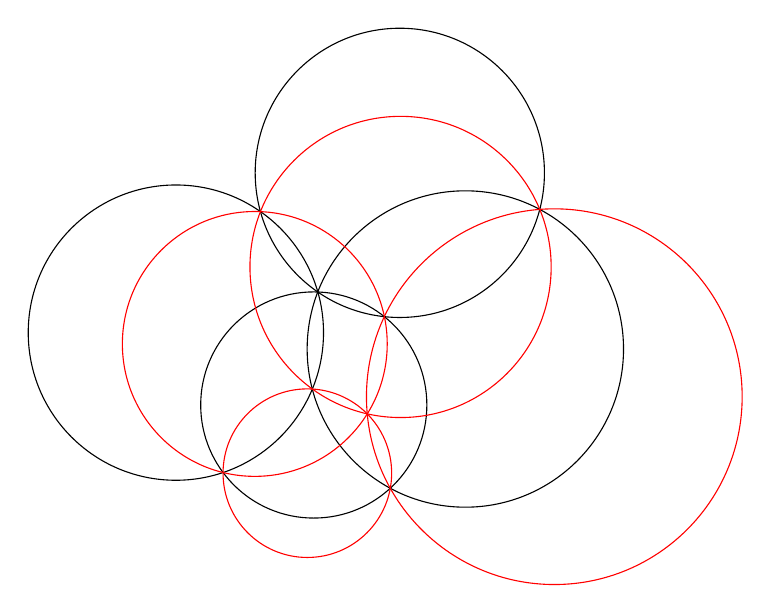
\begin{tikzpicture}[x=1pt,y=1pt]
\draw (153.95,-58.72) circle (52.26);
\draw (73.03,-116.45) circle (53.35);
\draw (177.63,-122.37) circle (57.16);
\draw (122.86,-142.60) circle (40.86);
\draw[red] (154.22,-92.72) circle (54.42);
\draw[red] (101.55,-120.54) circle (47.85);
\draw[red] (209.78,-139.60) circle (67.88);
\draw[red] (120.54,-167.24) circle (30.46);
\end{tikzpicture}
\end{document}
